\documentclass{exam}
\usepackage[utf8]{inputenc}
\usepackage{lmodern}
\usepackage{microtype}

% \usepackage[parfill]{parskip}
\usepackage[dvipsnames]{xcolor}
\usepackage{amsmath}
\usepackage{amsfonts}
\usepackage{amsthm}
\usepackage{siunitx}
\DeclareSIUnit\year{yr}
\DeclareSIUnit\foot{ft}
\DeclareSIUnit\litre{\liter}

\usepackage{skull}

\usepackage{pgfplots}
\usepgfplotslibrary{polar}
\pgfplotsset{compat=1.11}
\usepgfplotslibrary{statistics}
\usepackage{graphicx}
\usepackage{sidecap}
\sidecaptionvpos{figure}{c}
\usepackage{float}
\usepackage{gensymb}
\usepackage{tkz-euclide}
\usetkzobj{all}
\usepackage{commath}
\usepackage{hyperref}
\usepackage{enumitem}
\usepackage{wasysym}
\usepackage{multicol}
\usepackage{mathtools}
\usepackage{tcolorbox}
\usepackage{tabularx}
\usepackage[version=4]{mhchem}
\usepackage{changepage}
\usepackage{listings}
\lstset{basicstyle=\ttfamily\linespread{0.8}\small}

\renewcommand*{\thefootnote}{\fnsymbol{footnote}}

\newtheorem*{thm}{Theorem}
\newtheorem*{iden}{Identity}
\newtheorem*{lemma}{Lemma}
\newtheorem{obs}{Observation}
\theoremstyle{definition}
\newtheorem*{defn}{Definition}
\newtheorem*{ex}{Example}
\newtheorem{con}{Construction}
\newtheorem*{alg}{Algorithm}

\newtheoremstyle{break}
  {\topsep}{\topsep}%
  {\itshape}{}%
  {\bfseries}{}%
  {\newline}{}%
\theoremstyle{break}
\newtheorem*{bthm}{Theorem}

% russian integral
\usepackage{scalerel}
\DeclareMathOperator*{\rint}{\scalerel*{\rotatebox{17}{$\!\int\!$}}{\int}}

% \DeclareMathOperator*{\rint}{\int}

\pgfplotsset{vasymptote/.style={
    before end axis/.append code={
        \draw[densely dashed] ({rel axis cs:0,0} -| {axis cs:#1,0})
        -- ({rel axis cs:0,1} -| {axis cs:#1,0});
    }
}}

% \pointsinrightmargin
\boxedpoints
\pointname{}

\newcommand{\questioA}{\question[\texttt{\textbf{\color{Cerulean} A}}]}
\newcommand{\questioM}{\question[\texttt{\textbf{\color{PineGreen} M}}]}
\newcommand{\questioE}{\question[\texttt{\textbf{\color{WildStrawberry} E}}]}
\newcommand{\questioS}{\question[\texttt{\textbf{\color{Goldenrod} S}}]}
\newcommand{\questioO}{\question[\texttt{\textbf{\color{BurntOrange} O}}]}

\newcommand{\parA}{\part[\texttt{\textbf{\color{Cerulean} A}}]}
\newcommand{\parM}{\part[\texttt{\textbf{\color{PineGreen} M}}]}
\newcommand{\parE}{\part[\texttt{\textbf{\color{WildStrawberry} E}}]}
\newcommand{\parS}{\part[\texttt{\textbf{\color{Goldenrod} S}}]}
\newcommand{\parO}{\part[\texttt{\textbf{\color{BurntOrange} O}}]}

\newcommand{\subparA}{\subpart[\texttt{\textbf{\color{Cerulean} A}}]}
\newcommand{\subparM}{\subpart[\texttt{\textbf{\color{PineGreen} M}}]}
\newcommand{\subparE}{\subpart[\texttt{\textbf{\color{WildStrawberry} E}}]}
\newcommand{\subparS}{\subpart[\texttt{\textbf{\color{Goldenrod} S}}]}
\newcommand{\subparO}{\subpart[\texttt{\textbf{\color{BurntOrange} O}}]}

\newcommand{\mainHeader}[2]{\section*{NCEA Level 2 Mathematics\\#1. #2}}
\newcommand{\mainHeaderHw}[2]{\section*{NCEA Level 2 Mathematics (Homework)\\#1. #2}}
\newcommand{\seealso}[1]{\begin{center}\emph{See also #1.}\end{center}}
\newcommand{\drills}[1]{\begin{center}\emph{Drill problems: #1.}\end{center}}
\newcommand{\basedon}[1]{\begin{center}\emph{Notes largely based on #1.}\end{center}}


\begin{document}

\mainHeader{4}{Functions}
One of the most fundamental concepts in mathematics is that of a function. A function is a relationship between
two sets of things, called the \textit{range} and the \textit{domain}, such that everything in the range is
related to exactly one thing in the domain.

If $ f $ is a function, and it relates $ x $ to $ y $, then we write $ f(x) = y $. In this notation, $ x $ is the \emph{argument} or \emph{input}
and $ y $ is the \emph{result} or \emph{output}.

The above expression $ f(x) = y $ is suggestive: we can graph functions by graphing every pair of numbers $ (x,y) $
which satisfies this equation.

\begin{ex}\leavevmode
  \begin{enumerate}
    \item Suppose for every number $ n $ we associate its double, $ 2n $. This is a perfectly good function,
          which we can call $ f $: then $ f(n) = 2n $, and $ f(2) = 2 \cdot 2 = 4 $.
          \begin{center}
            \fbox{\begin{tikzpicture}
              \begin{axis}[
                scale = .8,
                axis lines = center,
                xlabel = $ n $,
                ylabel = $ f(n) $
              ]
                \addplot[domain = -5:5, color = red] {2*x};
              \end{axis}
            \end{tikzpicture}}
          \end{center}
    \item Suppose for every number $ x $ we associate the number which, when squared, gives $ x $. This is \emph{not}
          a well-defined function: for example, what number do we associate with $4$: $2$, or $ - 2 $? What number
          do we associate with $ -1 $?
    \item On the other hand, suppose for every positive number $ x $ we associate its positive square root. This time
          we do have a well-defined function. Note that its domain and range are both the positive numbers, and for every
          number in the domain there is precisely one number in the range.
          \begin{center}
            \fbox{\begin{tikzpicture}
              \begin{axis}[
                scale = .8,
                axis lines = center,
                xlabel = $ x $,
                ylabel = $ \sqrt{x} $,
                xmin = -5,
                ymax = 27
              ]
                \addplot[domain = 0:27, color = orange] {sqrt(x)};
              \end{axis}
            \end{tikzpicture}}
          \end{center}
    \clearpage
    \item Let $ g(x) = x^2 $. This is also a perfectly good function; every number has exactly one square. Note that $ g(-2) = g(2) = 4 $;
          this is allowed, but if a function $ f $ has the property that if $ x $ and $ y $ are different then $ f(x) \neq f(y) $ then $ f $
          is called one-to-one. The functions in (1) and (3) above are both one-to-one.
          \begin{center}
            \fbox{\begin{tikzpicture}
              \begin{axis}[
                scale = .8,
                axis lines = center,
                xlabel = $ x $,
                ylabel = $ g(x) $,
              ]
                \addplot[domain = -5:5, color = blue] {x^2};
              \end{axis}
            \end{tikzpicture}}
          \end{center}
          Notice that this is a square root on its side... can you explain why?
  \end{enumerate}
\end{ex}

One-to-one functions are useful, because they have an \emph{inverse}. That is, given any number in the \emph{range} we can find
the number in the \emph{domain} that maps to it. If $ f $ is a one-to-one function, then its inverse is written as $ f^{-1} $.

\begin{ex}\leavevmode
  \begin{enumerate}
    \item If $ f(x) = 2x $, then $ f^{-1}(x) = \frac{1}{2} x $.
    \item If $ g(x) = x^2 $, then $ g $ does not have an inverse over all the numbers; but if we restrict the domain of $ g $ to
          the positive numbers, then it does have an inverse $ g^{-1}(x) = +\sqrt{x} $.
    \item If $ h(x) = \sin x $ (and the range of $ x $ is restricted to $ 0 < x \leq 2\pi $) then $ h $ is a perfectly good function
          with range $ -1 \leq h(x) \leq 1 $; its inverse is $ \sin^{-1} $, which takes a triangle ratio and returns the appropriate angle.
  \end{enumerate}
\end{ex}

\clearpage
\subsection*{Questions}
\begin{questions}
  \question Justify the following statements with mathematical reasoning.
    \begin{parts}
      \part The graph of a function passes the vertical line test: any vertical line drawn on the graph crosses the function in at most one point.
      \part The graph of a one-to-one function passes the horizontal line test: any horizontal line drawn on the graph crosses the function in at most one point.
      \part The graph of the inverse of a function is the reflection of the graph of the function across the line $ x = y $.
      \part If we define $ f $ by
            \begin{displaymath}
              f(x) = \begin{cases} x &\text{ if } x \geq 0 \\ -x & \text{ if } x < 0 \end{cases}
            \end{displaymath}
            then $ f $ is a function but it is not one-to-one.
      \part If $ f $ and $ g $ are functions, and the range of $ g $ is the same as the domain of $ f $, and we define a new function $ (f \circ g) $
            by $ (f \circ g)(x) = f(g(x)) $, then $ (f \circ g) $ is a function with the same range as $f $ and the same domain as $ g $.
    \end{parts}
  \question The following define functions only if they have a domain which is restricted. What is the largest possible domain for each, so that
            they are still functions? What is the range of each?
    \begin{parts}
      \part $ f(x) = 1/x $
      \part $ g(\theta) = \tan \theta $
      \part $ h(x) = \left(\dfrac{x}{x - 2}\right)^2 $
    \end{parts}
  \question Which of the following graphs are graphs of functions? Of those, which are one-to-one?
    \begin{parts}
      \begin{minipage}{0.33\linewidth}
      \part \begin{center}
              \fbox{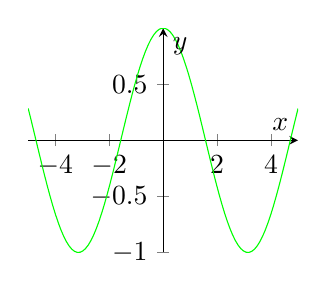
\begin{tikzpicture}
                \begin{axis}[
                  scale = .5,
                  axis lines = center,
                  xlabel = $ x $,
                  ylabel = $ y $,
                ]
                  \addplot[domain = -5:5, color = green, samples = 100] {cos(deg(x))};
                \end{axis}
              \end{tikzpicture}}
            \end{center}
      \end{minipage}
      \begin{minipage}{0.33\linewidth}
      \part \begin{center}
              \fbox{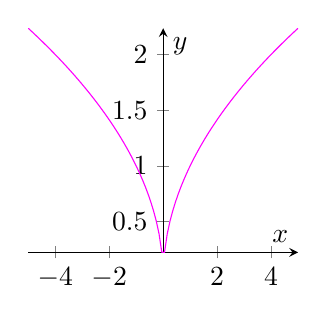
\begin{tikzpicture}
                \begin{axis}[
                  scale = .5,
                  axis lines = center,
                  xlabel = $ x $,
                  ylabel = $ y $,
                ]
                  \addplot[domain = -5:5, color = Fuchsia, samples = 100] {sqrt(abs(x))};
                \end{axis}
              \end{tikzpicture}}
            \end{center}
      \end{minipage}
      \begin{minipage}{0.33\linewidth}
      \part \begin{center}
              \fbox{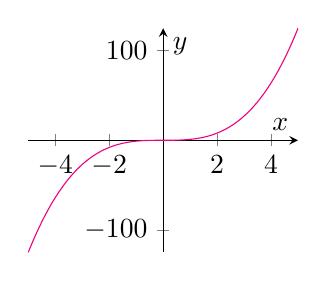
\begin{tikzpicture}
                \begin{axis}[
                  scale = .5,
                  axis lines = center,
                  xlabel = $ x $,
                  ylabel = $ y $,
                ]
                  \addplot[domain = -5:5, color = RubineRed, samples = 100] {x^3};
                \end{axis}
              \end{tikzpicture}}
            \end{center}
      \end{minipage}
      \begin{minipage}{0.33\linewidth}
      \part \begin{center}
              \fbox{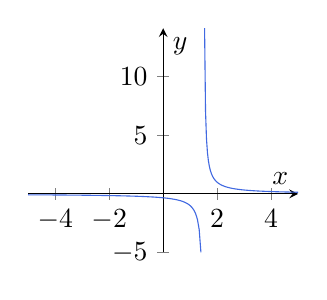
\begin{tikzpicture}
                \begin{axis}[
                  scale = .5,
                  axis lines = center,
                  xlabel = $ x $,
                  ylabel = $ y $,
                ]
                  \addplot[domain = -5:1.4, color = RoyalBlue, samples = 100] {1/(2*x - 3)};
                  \addplot[domain = 1.5:5, color = RoyalBlue, samples = 100] {1/(2*x - 3)};
                \end{axis}
              \end{tikzpicture}}
            \end{center}
      \end{minipage}
      \begin{minipage}{0.33\linewidth}
      \part \begin{center}
              \fbox{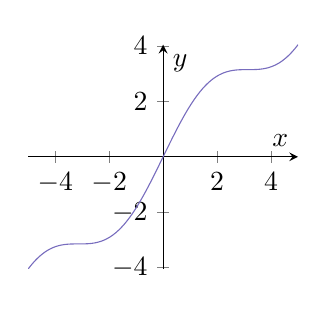
\begin{tikzpicture}
                \begin{axis}[
                  scale = .5,
                  axis lines = center,
                  xlabel = $ x $,
                  ylabel = $ y $,
                ]
                  \addplot[domain = -5:5, color = Periwinkle, samples = 100] {sin(deg(x)) + x};
                \end{axis}
              \end{tikzpicture}}
            \end{center}
      \end{minipage}
      \begin{minipage}{0.33\linewidth}
      \part \begin{center}
              \fbox{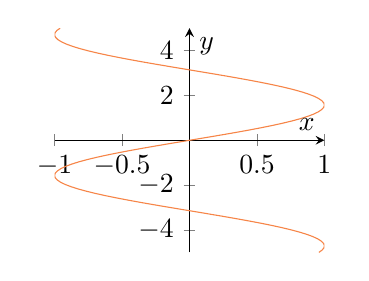
\begin{tikzpicture}
                \begin{axis}[
                  scale = .5,
                  axis lines = center,
                  xlabel = $ x $,
                  ylabel = $ y $,
                ]
                  \addplot[domain = -5:5, color = Peach, samples = 100] (sin(deg(x)),x);
                \end{axis}
              \end{tikzpicture}}
            \end{center}
      \end{minipage}
      \begin{minipage}{0.33\linewidth}
      \part \begin{center}
              \fbox{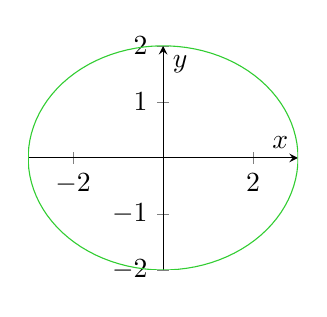
\begin{tikzpicture}
                \begin{axis}[
                  scale = .5,
                  axis lines = center,
                  xlabel = $ x $,
                  ylabel = $ y $,
                ]
                  \addplot[domain = 0:360, color = LimeGreen, samples = 100] ({3*cos(x)}, {2*sin(x)});
                \end{axis}
              \end{tikzpicture}}
            \end{center}
      \end{minipage}
      \begin{minipage}{0.33\linewidth}
      \part \begin{center}
              \fbox{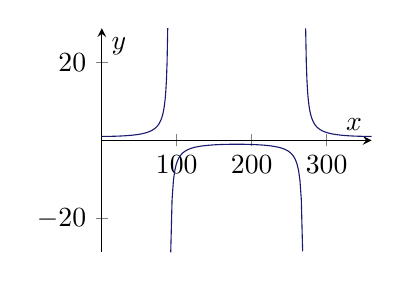
\begin{tikzpicture}
                \begin{axis}[
                  scale = .5,
                  axis lines = center,
                  xlabel = $ x $,
                  ylabel = $ y $,
                ]
                  \addplot[domain = 0:88, color = MidnightBlue, samples = 100] {sec(x)};
                  \addplot[domain = 92:268, color = MidnightBlue, samples = 100] {sec(x)};
                  \addplot[domain = 272:360, color = MidnightBlue, samples = 100] {sec(x)};
                \end{axis}
              \end{tikzpicture}}
            \end{center}
      \end{minipage}
      \begin{minipage}{0.33\linewidth}
      \part \begin{center}
              \fbox{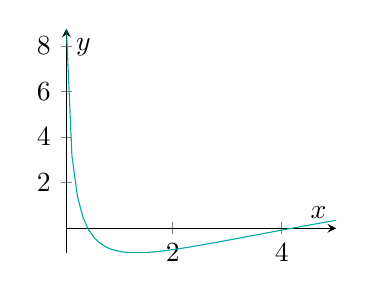
\begin{tikzpicture}
                \begin{axis}[
                  scale = .5,
                  axis lines = center,
                  xlabel = $ x $,
                  ylabel = $ y $,
                ]
                  \addplot[domain = -5:5, color = Emerald, samples = 100] {(ln(x))^2 - sqrt(x)};
                \end{axis}
              \end{tikzpicture}}
            \end{center}
      \end{minipage}
    \end{parts}
  \question We will now look at shifting graphs around.
    \begin{parts}
      \part Graph $ f $, if $ f(x) = x^2 $.
      \part On the same paper, graph $ f(x - 1) $ and $ f(x + 1) $.
      \part Graph $ f(x) - 1 $ and $ f(x) + 1 $.
      \part Graph $ 2 f(x) $ and $ f(2x) $.
      \part Make a conjecture about the relationship between the following graphs, if $ f $ is now any function and $ a $, $ b $, $ c $, and $ d $ are any numbers:
        \begin{subparts}
          \subpart $ y = f(x) $
          \subpart $ y = f(x + a) $
          \subpart $ y = f(x) + b $
          \subpart $ y = c f(x) $
          \subpart $ y = f(dx) $
        \end{subparts}
      \part Explain intuitively why, when we add numbers inside the function argument, the graph shifts `the wrong way'.
      \part Graph $ y = 3\sin(\frac{1}{2} x + 1) - 2 $.
    \end{parts}
  \question If I take $ y = x^2 $ and I want to shift and stretch its graph so that the vertex is sitting at $ (-2, 3) $ and it goes through $ (1,1) $, can I do
            that? If so, what is the equation of the function that gives me the new graph?
  \question The following graph is of the function $ c $, where $ c(x) $ is the proportion of a particular chemical species in solution
            at pH $ x $ (pH is, roughly speaking, a measure of acidity). \footnote{From \emph{Quantitative Chemical Analysis}, 7th edition,
            by Daniel Harris (page 233).}
            \begin{center}
            \fbox{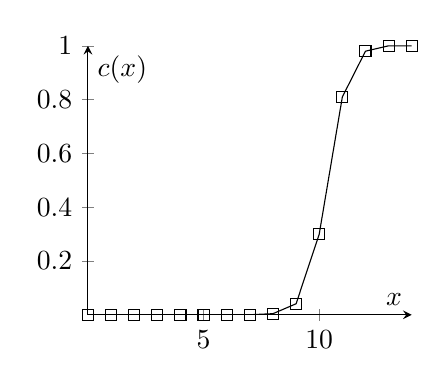
\begin{tikzpicture}
              \begin{axis}[
                /pgf/number format/1000 sep={},
                scale = .6,
                axis lines = center,
                xlabel = $ x $,
                ylabel = $ c(x) $
              ]
                \addplot[mark = square] coordinates{(0,{1.3e-23})(1,{1.4e-18})(2,{2.6e-14})(3,{2.1e-11})(4,{3.0e-9})(5,{2.9e-7})(6,{1.8e-5})(7,{2.8e-4})(8,{4.2e-3})(9,0.041)(10,0.30)(11,0.81)(12,0.98)(13,1.00)(14,1.00)};
              \end{axis}
            \end{tikzpicture}}
          \end{center}
    \begin{parts}
      \part Is this function invertible? That is, if I measure the concentration of this species at any point, can I identify precisely what the pH of
            the solution is?
      \part Explain why knowing the proportion of a chemical species in water at a given pH might be useful; why is mathematical modelling useful
            in such a situation?
    \end{parts}
  \clearpage
  \question The following graph is of the function $ P $, where $ P(x) $ is the population of the Greater Wellington region in the year $ x $.\footnote{Statistics
            are the Statistics NZ `Subnational population estimates (RC, AU), by age and sex, at 30 June 1996, 2001, 2006-17 (2017 boundaries)' (retrieved
            19 June 2018).} Note that the $ y$-axis does \emph{not} start at zero, and is given in units of hundreds of thousands.
            \begin{center}
            \fbox{\begin{tikzpicture}
              \begin{axis}[
                /pgf/number format/1000 sep={},
                axis lines = center,
                xlabel = $ x $,
                ylabel = $ P(x) $,
                xmin = 1995, xmax = 2020,
                ymax = 540000
              ]
                \addplot[mark = square] coordinates{(1996,426900)(2001,440200)(2006,466300)(2007,469300)(2008,471800)(2009,475600)(2010,479400)(2011,483400)(2012,485100)(2013,486700)(2014,491400)(2015,496900)(2016,504900)(2017,513900)};
              \end{axis}
            \end{tikzpicture}}
          \end{center}
    \begin{parts}
      \part Explain why extrapolating using this graph to find $ P(2020) $ is probably justified.
      \part Give an example of a function where the values of the function above any point cannot be extrapolated from knowing the values of the
            function before the point. Do you think that extrapolation is normally possible for mathematical models of the natural world?
      \part Describe how the rate of population growth changes as we move forwards in time from 1996 to 2017.
      \part Given the real-world context of this graph, how would you expect the slope of the graph to change:
        \begin{subparts}
          \subpart in the medium term (up to, say, 2040), and
          \subpart in the long term (say around the year 2100).
        \end{subparts}
    \end{parts}
\end{questions}

\end{document}
